\documentclass[11pt]{article}
\usepackage{graphicx}
\graphicspath{{./Secoes/Figuras/Photos/}}
\usepackage[utf8]{inputenc} % Para aceitar acentos
\usepackage[T1]{fontenc}    % Para renderizar fontes com acentos corretamente
\usepackage[brazil]{babel}  % Para português (hifenização, datas, etc.)
\usepackage[a4paper, margin=2.5cm]{geometry} % Ajusta a largura da folha
\usepackage[ruled,vlined, linesnumbered]{algorithm2e}% Escrever pseudocódigo
\usepackage{amsmath}  % Suporte matemático extra
\usepackage{amssymb}  % Define o \mathbb
\usepackage{hyperref}
\usepackage{xcolor}
\usepackage{adjustbox}
\usepackage{setspace}

\usepackage{float}
\usepackage{multirow}
\usepackage[table]{xcolor}

\newcommand{\blue}[1]{\textcolor{blue}{#1}}
\newcommand{\red}[1]{\textcolor{red}{#1}}


\usepackage[utf8]{inputenc}
\usepackage[T1]{fontenc}
\usepackage[brazil]{babel}
\usepackage{pgfgantt}
\usepackage{geometry}
\usepackage{amssymb}
\usepackage{caption}
\captionsetup{
    justification=raggedright,
    singlelinecheck=false
}
\usepackage{subcaption}

\usepackage{tikz}
\usetikzlibrary{positioning, arrows.meta}

\geometry{margin=2.5cm}

\setlength{\parindent}{1.25cm}
\setlength{\parskip}{4pt}

\title{Projeto de pesquisa - Problema da compra mínima}
\author{Antônio Erick Freitas Ferreira \\
        \small Instituto de Computação - Unicamp - São Paulo - Brasil
}

\begin{document}

\newcommand{\conjuntoItens}{

\begin{tikzpicture}[
    thick,
    item/.style={circle, draw, minimum size=9mm},
    buyer/.style={circle, draw,  minimum size=9mm}
]
    % Itens
    \node[item] (i1) at (0,2) {$i_1$};
    \node[item] (i2) at (0,0) {$i_2$};
    \node[item] (i3) at (0,-2) {$i_3$};
    \node[item] (i3) at (0,-4) {$i_4$};

\end{tikzpicture}
}


\newcommand{\conjuntoCompradores}{

\begin{tikzpicture}[
    thick,
    item/.style={circle, draw, minimum size=9mm},
    buyer/.style={circle, draw,  minimum size=9mm}
]

    % Compradores
    \node[buyer] (b1) at (5,2) {$b_1$};
    \node[buyer] (b2) at (5,0) {$b_2$};
    \node[buyer] (b2) at (5,-2) {$b_3$};
    \node[buyer] (b2) at (5,-4) {$b_4$};

\end{tikzpicture}
}


\newcommand{\conjuntoItensValorados}{

\begin{tikzpicture}[
    thick,
    item/.style={circle, draw, minimum size=9mm},
    buyer/.style={circle, draw,  minimum size=9mm},
    scale=0.8
]
    % Itens
    \node[item] (i1) at (0,2) {$i_1$};
    \node[item] (i2) at (0,0) {$i_2$};
    \node[item] (i3) at (0,-2) {$i_3$};
    \node[item] (i4) at (0,-4) {$i_4$};

    % Compradores
    \node[buyer] (b1) at (5,2) {$b_1$};
    \node[buyer] (b2) at (5,0) {$b_2$};
    \node[buyer] (b3) at (5,-2) {$b_3$};
    \node[buyer] (b4) at (5,-4) {$b_4$};

    % Arestas
    \draw (b1) --node[pos=0.2, fill=white]{3} (i1);
    \draw (b1) --node[pos=0.2, fill=white]{4} (i2);
    \draw (b1) --node[pos=0.215, fill=white]{2} (i3);

    \draw (b2) --node[pos=0.2, fill=white]{5} (i2);
    \draw (b2) --node[pos=0.2, fill=white]{6} (i3);
    \draw (b2) --node[pos=0.215, fill=white]{3} (i4);

    \draw (b3) --node[pos=0.2, fill=white]{5} (i3);
    \draw (b3) --node[pos=0.2, fill=white]{2} (i4);

    \draw (b4) --node[pos=0.2, fill=white]{2} (i4);
    % \draw (i2) -- (b2);
    % \draw (i3) -- (b2);
\end{tikzpicture}
}

\newcommand{\conjuntoItensPrecificados}{

\begin{tikzpicture}[
    thick,
    item/.style={circle, draw, minimum size=9mm},
    buyer/.style={circle, draw,  minimum size=9mm},
    scale=0.8
]
    % Itens
    \node[item, label=below:{$p_1 = 3$}] (i1) at (0,2) {$i_1$};
    \node[item, label=below:{$p_2 = 5$}] (i2) at (0,0) {$i_2$};
    \node[item, label=below:{$p_3 = 5$}] (i3) at (0,-2) {$i_3$};
    \node[item, label=below:{$p_4 = 3$}] (i4) at (0,-4) {$i_4$};

    % Compradores
    \node[buyer] (b1) at (5,2) {$b_1$};
    \node[buyer] (b2) at (5,0) {$b_2$};
    \node[buyer] (b3) at (5,-2) {$b_3$};
    \node[buyer] (b4) at (5,-4) {$b_4$};

    % Arestas
    \draw (i1) -- (b1);
    \draw (i4) -- (b2);
    \draw (i3) -- (b3);


    % \draw[dashed, thick] (b1) -- (i2);
    % \draw[dashed, thick] (b1) -- (i3);

    \draw[dashed, thick] (b2) -- (i2);
    \draw[dashed, thick] (b2) --(i3);

    % \draw[dashed, thick] (b3) --(i4);

    % \draw[dashed, thick] (b4) -- (i4);
    
\end{tikzpicture}
}


\newcommand{\fluxograma}{
    \begin{tikzpicture}[
        every node/.style={draw, minimum height=1.2cm, minimum width=3.8cm, font=\ttfamily, align=center},
        decision/.style={aspect=2, draw, minimum height=1.5cm, inner sep=0pt},
        arrow/.style={->, thick},
        node distance=1.2cm and 2cm
    ]
        % Nós
        \node (begin) at (-10,-1.5) [circle, draw, minimum size=1.2cm] {Início};
        \node (genKeys) at (-5,-1.5) {Gerar a população\\ inicial};
        \node (fitness) at (-5, -4) {Avaliação de \\ fitness};
        \node (checkStop) at (4, -4) [diamond, decision, fill=gray!20] {Critério de parada\\ satisfeito?};
        \node (selection) at (4, -8) {Seleção};
        \node (crossover) at (-1.5, -8) {Cruzamento};
        \node (mutation) at (-7.5, -8) {Mutação};
        \node (elitism) at (-13.5, -8) {Elitismo};
        \node (newPop) at (-13.5, -4) {Nova população};
        \node (final) at (4, -1) [circle, draw, minimum size=1.2cm] {Fim};
        
    \begin{scope}[
              every node/.style={fill=white,circle}, arrow/.style={->,ultra thick}]
        % Conexões
        \draw[arrow] (begin) -- (genKeys);
        \draw[arrow] (genKeys) -- (fitness);
        \draw[arrow] (fitness) -- (checkStop);
        \draw[arrow] (checkStop) --node[right]{Não} (selection);
        \draw[arrow] (selection) -- (crossover);
        \draw[arrow] (crossover) -- (mutation);
        \draw[arrow] (mutation) -- (elitism);
        \draw[arrow] (elitism) -- (newPop);
        \draw[arrow] (newPop) -- (fitness);
        \draw[arrow] (checkStop) -- node[right]{Sim} (final);
        
    \end{scope}
    \end{tikzpicture}
}

\newcommand{\fluxogramaBRKGA}{
    \begin{tikzpicture}[
        every node/.style={draw, minimum height=1.2cm, minimum width=3.8cm, font=\ttfamily, align=center},
        decision/.style={aspect=2, draw, minimum height=1.5cm, inner sep=0pt},
        arrow/.style={->, thick},
        node distance=1.2cm and 2cm
    ]
        % Nós
        \node (begin) at (-10,-1.5) [circle, draw, minimum size=1.2cm] {Início};
        \node (genKeys) at (-5,-1.5) {Gerar os vetores\\ de chaves aleatórias};
        \node (fitness) at (-5, -4) {Decodificar cada vetor \\ de chave aleatória};
        \node (checkStop) at (4, -4) [diamond, decision, fill=gray!20] {Regra de parada\\ satisfeito?};
        \node (selection) at (4, -8) {Classificar indivíduos\\como elite ou não-elite};
        \node (crossover) at (-2, -8) {Copiar os elite para\\a próxima geração};
        \node (mutation) at (-7.5, -8) {Criar mutantes para\\próxima geração};
        \node (elitism) at (-13.5, -8) {Gerar descendentes para\\a próxima geração};
        \node (newPop) at (-13.5, -4) {Nova população};
        \node (final) at (4, -1) [circle, draw, minimum size=1.2cm] {Fim};
        
    \begin{scope}[
              every node/.style={fill=white,circle}, arrow/.style={->,ultra thick}]
        % Conexões
        \draw[arrow] (begin) -- (genKeys);
        \draw[arrow] (genKeys) -- (fitness);
        \draw[arrow] (fitness) -- (checkStop);
        \draw[arrow] (checkStop) --node[right]{Não} (selection);
        \draw[arrow] (selection) -- (crossover);
        \draw[arrow] (crossover) -- (mutation);
        \draw[arrow] (mutation) -- (elitism);
        \draw[arrow] (elitism) -- (newPop);
        \draw[arrow] (newPop) -- (fitness);
        \draw[arrow] (checkStop) -- node[right]{Sim} (final);
        
    \end{scope}
    \end{tikzpicture}
}

% \begin{titlepage}
    {
        \centering
    
        {\large Universidade Estadual de Campinas \\}
        {\large Instituto de Computação \\}
        
        {\LARGE \textbf{O Problema da Compra Mínima: Heurísticas baseadas em Chaves Aleatórias e Otimização de Formulações Existentes} \\[1cm]}
        
        {\large Candidato: Antônio Erick Freitas Ferreira \\}

        {\large Orientador: Rafael Crivellari Saliba Schouery}
        
    }

    \begin{abstract}

O problema de determinar preços para um conjunto de produtos constitui um desafio central em cenários de mercados competitivos, gerando um dilema econômico: preços elevados maximizam a receita unitária, o que, consequentemente, reduz o mercado consumidor, enquanto preços baixos expandem o volume de vendas em detrimento da margem de lucro por transação. Diante disso, este trabalho estuda o \emph{Problema da Compra Mínima} (PCmin), que consiste em maximizar a receita total de um vendedor por meio da precificação de um conjunto de itens. Nesse cenário, assume-se que o valor máximo que cada comprador está disposto a pagar é previamente conhecido. Além disso, adota-se a hipótese de demanda unitária. Dessa forma, cada comprador adquire apenas o item mais barato dentre aqueles de seu interesse, ou opta por não comprar nada caso todos os preços excedam sua disposição a pagar. Embora o PCmin tenha recebido atenção crescente na literatura, sua investigação sob a perspectiva de algoritmos exatos ainda é limitada. As formulações matemáticas existentes apresentam restrições quanto à eficiência computacional, especialmente na resolução de instâncias de maior porte. Nesse contexto, identifica-se uma lacuna no desenvolvimento de métodos capazes de ampliar a escalabilidade e reduzir os tempos de solução do problema. Assim, este projeto propõe o aprimoramento de formulações de Programação Linear Inteira já existentes, bem como o desenvolvimento de abordagens heurísticas, com o objetivo de obter soluções de alta qualidade para instâncias de diferentes dimensões em tempos computacionais viáveis.


\end{abstract}



    {\textbf{Palavras-chave:} Otimização combinatória, precificação, programação linear inteira, heurística.}
% \end{titlepage}
\newpage

% \tableofcontents
% \newpage

\section{Introdução}

Relações comerciais fazem parte do cotidiano e envolvem, de maneira recorrente, decisões sobre preços e consumo. De modo geral, um vendedor disponibiliza seus produtos por determinados valores, enquanto os compradores decidem adquiri-los ou não com base em sua disposição a pagar. Em mercados cada vez mais competitivos, a definição de preços deixa de ser uma tarefa meramente operacional e passa a constituir uma decisão estratégica, capaz de impactar diretamente a receita obtida. Nesse contexto, surge uma questão central: como precificar um conjunto de produtos de forma a maximizar o retorno financeiro?

Esse tipo de situação se insere em uma classe mais ampla de problemas conhecidos como \textit{Problemas de Precificação} (PP), nos quais um vendedor deve determinar os preços de seus produtos de modo a maximizar a receita total obtida com as vendas. Essa decisão é particularmente desafiadora porque o preço de cada item influencia simultaneamente o valor arrecadado por unidade e o conjunto de consumidores dispostos a adquiri-lo, evidenciando a necessidade de equilibrar competitividade e rentabilidade~\cite{smith1986}. Problemas de precificação estão presentes em diversos setores da economia e têm sido amplamente investigados na literatura em razão de sua elevada relevância prática e aplicabilidade em contextos reais~\cite{aggarwal2004,venkatesan2005,shmuel1984,shmuel1987,smith1986}.

No contexto de problemas de precificação não paramétrica com múltiplos itens e múltiplos compradores, Rusmevichientong et al.~\cite{rusmevichientong2006} formalizaram um arcabouço geral no qual o vendedor conhece previamente as valorações dos compradores para os itens disponíveis e deve definir os preços de forma a maximizar a receita. Nesse arcabouço, diferentes variantes foram propostas para representar distintos comportamentos de compra. Entre elas, destacam-se o \textit{Problema da Compra Máxima} (PCmax), no qual o comprador seleciona o item viável de maior preço, e o \textit{Problema da Compra por Preferência} (PCrank), em que o comprador escolhe, dentre os itens viáveis, aquele que ocupa a posição mais alta em sua ordem de preferência.

Dentre essas variantes, este trabalho concentra-se no \textit{Problema da Compra Mínima} (PCmin). Nessa variante, o vendedor deve definir os preços de um conjunto de itens de modo a maximizar sua receita total, assumindo que cada comprador adquire, dentre os itens viáveis, aquele de menor preço. Um item é considerado viável para um comprador quando seu preço não excede a valoração atribuída a esse item por esse comprador. Caso nenhum item satisfaça essa condição, nenhuma compra é realizada. Essa hipótese de comportamento torna o PCmin particularmente relevante do ponto de vista prático, uma vez que, em diversos contextos, consumidores tendem a optar pelo item de menor preço dentre alternativas que consideram aceitáveis ou substitutos próximos.

De maneira formal, o PCmin foi definido por Rusmevichientong como segue. Seja $I$ um conjunto de itens, $B$ um conjunto de compradores e $V$ uma matriz de valorações, em que cada elemento $v_{ib} \in V$ representa a valoração do comprador $b \in B$ para o item $i \in I$. O problema consiste em determinar um conjunto de preços $P$, no qual cada elemento $p_i \in P$ corresponde ao preço atribuído ao item $i$, de modo a maximizar a receita total do vendedor. Assume-se, adicionalmente, que o comportamento dos compradores é conhecido e segue uma regra determinística: cada comprador $b \in B$ adquire, dentre os itens viáveis, aquele de menor preço. Em outras palavras, o comprador escolhe um item $i \in I$ tal que $p_i \leq v_{ib}$ e, para todo item $j \in I$ satisfazendo $p_j \leq v_{jb}$, vale $p_i \leq p_j$. Caso não exista item viável, o comprador não realiza compra.

Essa hipótese de comportamento torna o PCmin particularmente relevante do ponto de vista prático, uma vez que, em diversos contextos reais, consumidores tendem a optar pelo item de menor preço dentre aqueles que consideram aceitáveis ou de seu interesse. Embora fatores como marca, qualidade percebida e preferências individuais também possam influenciar a decisão de compra, o critério de menor preço frequentemente exerce papel determinante, especialmente em mercados com produtos substitutos ou de baixa diferenciação.

A Figura~\ref{fig:exemploPCmin} apresenta um exemplo ilustrativo de uma instância do PCmin. Na subfigura~(a), são representadas as relações de valoração entre os itens e os compradores por meio de um grafo bipartido, no qual cada aresta ponderada indica a valoração atribuída por um comprador a um determinado item. Na subfigura~(b), são mostrados os preços atribuídos aos itens e as escolhas induzidas pela regra do problema. Nesse caso, cada comprador adquire o item de menor preço dentre aqueles de seu interesse cujo preço não excede sua respectiva valoração. Assim, observa-se que o comprador $b_1$ seleciona o item $i_1$, o comprador $b_2$ seleciona o item $i_4$, o comprador $b_3$ seleciona o item $i_3$, enquanto o comprador $b_4$ não realiza compra, uma vez que não há item viável disponível para ele.

\begin{figure}[H]
\centering

\begin{subfigure}[t]{0.45\textwidth}
    \centering
    \conjuntoItensValorados
    \caption{Relações de valoração entre itens e compradores, representadas pelas arestas ponderadas da matriz $V$.}
\end{subfigure}
\hfill
\begin{subfigure}[t]{0.45\textwidth}
    \centering
    \conjuntoItensPrecificados
    \caption{Preços atribuídos aos itens e seleção induzida dos compradores segundo a regra do PCmin.}
\end{subfigure}

\caption{Exemplo ilustrativo de uma instância do PCmin, com as valorações entre itens e compradores e a seleção induzida pelos preços atribuídos.}
\label{fig:exemploPCmin}
\end{figure}

No exemplo ilustrado na Figura~\ref{fig:exemploPCmin}, a solução apresentada gera uma receita total de 11 unidades monetárias, correspondente às compras realizadas por $b_1$, $b_2$ e $b_3$. Entretanto, esse conjunto de preços não é necessariamente ótimo. Alterações nos preços podem modificar o conjunto de itens viáveis para cada comprador e, consequentemente, alterar tanto a quantidade de vendas quanto a receita obtida por item. Assim, a definição dos preços envolve uma interação não trivial entre viabilidade de compra e retorno financeiro, o que justifica o uso de métodos de otimização para a resolução do PCmin.

No que se refere ao desenvolvimento teórico do PCmin, Rusmevichientong et al.~\cite{rusmevichientong2006} foram os primeiros a formalizar o problema no contexto de problemas de precificação não paramétrica com múltiplos itens e compradores. Além de introduzir o PCmin, os autores o inserem em uma família mais ampla de variantes de precificação, como o PCmax e o PCrank. Contudo, esse estudo possui caráter predominantemente conceitual, concentrando-se na definição do problema e em suas propriedades estruturais, sem avançar no desenvolvimento de formulações matemáticas ou métodos computacionais voltados à sua resolução prática.

Posteriormente, Briest e Krysta~\cite{briest2007} e Chalermsook et al.~\cite{chalermsook2012} aprofundaram a investigação teórica do PCmin ao estabelecer resultados de complexidade e aproximabilidade, evidenciando sua elevada dificuldade computacional. Esses trabalhos são fundamentais por consolidarem o entendimento de que o problema é NP-difícil e, portanto, desafiador sob a perspectiva algorítmica. Ainda assim, tais contribuições permanecem restritas ao campo teórico, sem propor formulações de Programação Linear Inteira Mista (PLIM), técnicas de fortalecimento ou abordagens heurísticas voltadas ao tratamento de instâncias práticas.

Mais recentemente, o trabalho de Catabriga~\cite{catabriga2025} representa um avanço importante ao investigar o PCmin sob a ótica da otimização exata. Nesse estudo, são propostas diferentes formulações de Programação Linear Inteira (PLI) e Programação Linear Inteira Mista (PLIM), além de técnicas de fortalecimento dos modelos e de uma avaliação computacional em distintas classes de instâncias. Embora os resultados evidenciem o potencial dessas abordagens para a resolução do problema, também revelam limitações de escalabilidade à medida que o porte das instâncias aumenta. Adicionalmente, até o momento, não foram identificadas na literatura abordagens heurísticas especificamente direcionadas à resolução de instâncias de grande porte do PCmin, em particular aquelas com mais de 1000 itens e/ou compradores, o que evidencia uma lacuna relevante no tratamento computacional do problema.

Nesse contexto, o presente trabalho posiciona-se como uma continuidade dessa linha de pesquisa, com o objetivo de contribuir para o avanço do estudo do PCmin sob a perspectiva computacional. Em particular, pretende-se investigar e aperfeiçoar formulações matemáticas existentes, por meio da análise de estratégias de fortalecimento da relaxação linear, eliminação de simetrias e redundâncias, redução do número de variáveis e restrições, bem como da proposição de reformulações que favoreçam o desempenho computacional de solucionadores de programação inteira, como o Gurobi~\cite{gurobi}. Adicionalmente, busca-se desenvolver e avaliar abordagens heurísticas voltadas à obtenção de soluções de boa qualidade para instâncias de grande porte, em especial aquelas com mais de 1000 itens e/ou compradores, em tempo computacional reduzido. Espera-se, assim, ampliar o conjunto de ferramentas disponíveis para a resolução eficiente do PCmin, tanto no âmbito de métodos exatos quanto no de estratégias aproximativas.
\section{Metodologia}

A presente seção descreve a metodologia adotada para o desenvolvimento deste trabalho, contemplando os principais fundamentos teóricos e as abordagens computacionais empregadas na modelagem e resolução do problema em estudo. Inicialmente, são apresentados os conceitos de Programação Linear e Programação Linear Inteira, que fornecem a base matemática para a formulação do problema. Em seguida, são discutidas metaheurísticas inspiradas em processos evolutivos, com ênfase nos Algoritmos Genéticos e em suas variações baseadas em chaves aleatórias. Depois, é introduzido o framework Random-Key Optimizer (RKO), que integra diferentes estratégias de busca em uma representação unificada, servindo como principal abordagem adotada neste trabalho. Por fim, é discutido as formluções matemáticas existentes para o PCmin.

\subsection{Programação Linear}

A \textit{Programação Linear} (PL) consiste em uma das técnicas mais tradicionais da Pesquisa Operacional, sendo empregada na modelagem e resolução de problemas de otimização nos quais se deseja maximizar ou minimizar uma função objetivo linear sujeita a um conjunto de restrições também lineares. Esse tipo de abordagem é amplamente aplicado em contextos como alocação de recursos, planejamento produtivo e problemas logísticos, nos quais as relações entre variáveis podem ser adequadamente descritas por funções lineares.

A formulação de um problema de PL baseia-se na construção de um modelo matemático que represente fielmente o sistema real. O termo “linear” indica que todas as relações envolvidas, tanto na função objetivo quanto nas restrições, são expressas por funções lineares. Já o termo “programação” deve ser entendido como planejamento, e não como programação computacional. Assim, a programação linear trata do planejamento de atividades com o intuito de alcançar um resultado ótimo, isto é, aquele que melhor atende ao objetivo definido dentro do conjunto de soluções viáveis~\cite{Hillier2013}.

Em um modelo de PL, assume-se que as variáveis de decisão pertencem ao conjunto dos números reais $\mathbb{R}$, isto é, são contínuas. As restrições do modelo delimitam a região factível, e uma solução é considerada viável se satisfaz todas essas restrições. A solução ótima corresponde à melhor solução viável segundo o critério estabelecido pela função objetivo. Quando expresso em sua forma canônica, o modelo de programação linear pode ser descrito como:

\[
    \begin{aligned}
    \text{max} \quad & z = c^T x \\
    \text{sujeito a} \quad & Ax \leq b \\
    & x \geq 0
    \end{aligned}
\]

em que:
\begin{itemize}
    \item $x \in \mathbb{R}^n$ representa o vetor de variáveis de decisão;
    \item $c \in \mathbb{R}^n$ contém os coeficientes da função objetivo;
    \item $A \in \mathbb{R}^{m \times n}$ é a matriz de coeficientes das restrições;
    \item $b \in \mathbb{R}^m$ representa os termos independentes das restrições;
    \item $z \in \mathbb{R}$ é o valor da função objetivo.
\end{itemize}

Um dos principais avanços na resolução de problemas de programação linear ocorreu em 1947, quando George Dantzig propôs o algoritmo simplex~\cite{Nash2000}. Trata-se de um método exato e iterativo que explora a estrutura geométrica do problema, percorrendo os vértices do politopo definido pelas restrições. A cada iteração, o método busca uma solução adjacente que melhore o valor da função objetivo, até que não seja mais possível obter ganhos adicionais, caracterizando assim a otimalidade da solução encontrada~\cite{Goldbarg2005}.

\subsubsection{Programação Linear Inteira}

A \textit{Programação Linear Inteira} (PLI) constitui uma extensão da programação linear, na qual se impõe que parte ou a totalidade das variáveis de decisão assumam valores inteiros. Essa restrição transforma o conjunto de soluções viáveis, que deixa de ser contínuo e passa a ser discreto, o que aumenta significativamente a complexidade do problema~\cite{Nemhauser1988}.

De acordo com Goldbarg~\cite{Goldbarg2005}, um problema é classificado como de \emph{Programação Inteira} (PI) quando ao menos uma variável de decisão está restrita a assumir valores discretos. Formalmente, isso implica que $x_i \in \mathbb{Z}$ para as variáveis sujeitas à integralidade. Apesar de sua formulação aparentemente simples, essa restrição torna o problema consideravelmente mais difícil do ponto de vista computacional, sendo, em geral, NP-difícil~\cite{Schrijver1986}.

Problemas de PLI são particularmente adequados para modelar situações em que as decisões envolvem quantidades indivisíveis, como seleção de projetos, definição de rotas, alocação de equipes ou decisões binárias. Para sua resolução, métodos clássicos de PL, como o simplex, não são suficientes, sendo necessário recorrer a técnicas mais elaboradas, como branch-and-bound~\cite{Wosley1998}, métodos de enumeração e abordagens híbridas como branch-and-cut~\cite{Bertsimas2005}.

Um conceito central nesse contexto é o \emph{relaxamento linear}, que consiste em remover temporariamente as restrições de integralidade, permitindo que as variáveis assumam valores contínuos. A solução desse problema relaxado fornece um limitante para o problema original: no caso de maximização, um limitante superior; e no caso de minimização, um limitante inferior. Caso a solução obtida seja inteira, ela também é ótima para o problema original~\cite{Nemhauser1988}.

O método de \emph{branch-and-bound} é uma das principais estratégias para resolver problemas de PLI. Sua ideia central é explorar sistematicamente o espaço de soluções por meio de uma árvore de busca. Inicialmente, resolve-se o relaxamento linear do problema. Caso a solução encontrada não seja inteira, o problema é particionado em subproblemas (ramificação), adicionando-se restrições que forçam determinadas variáveis a assumir valores inteiros específicos. Para cada subproblema, calcula-se um limitante por meio do relaxamento linear, permitindo descartar regiões do espaço de busca que não podem conter soluções melhores do que a já conhecida (delimitação). Esse processo é repetido até que todas as regiões relevantes sejam exploradas ou eliminadas.

Uma evolução importante dessa abordagem é o método de \emph{branch-and-price}, que combina a estratégia de branch-and-bound com técnicas de geração de colunas. Essa abordagem é particularmente útil em problemas com um número muito grande de variáveis, nos quais a formulação completa seria impraticável. Em vez de considerar todas as variáveis desde o início, o método resolve iterativamente versões restritas do problema, adicionando novas variáveis (colunas) apenas quando necessário, com base em problemas auxiliares de precificação. A integração entre a geração dinâmica de colunas e a estrutura de ramificação permite resolver instâncias de grande porte de forma mais eficiente, sendo amplamente utilizada em problemas clássicos como corte de estoque e roteamento de veículos.


\subsection{Algoritmo Genético}

A teoria da evolução das espécies, proposta por Charles Darwin em \emph{A Origem das Espécies}, estabelece que os organismos evoluem ao longo de gerações por meio do mecanismo de seleção natural, frequentemente descrito como a sobrevivência dos mais aptos~\cite{Sivanandam2007}. Nesse processo, características que conferem vantagens adaptativas tendem a ser preservadas e propagadas, resultando, ao longo do tempo, em soluções altamente eficientes do ponto de vista biológico. Exemplos dessa eficiência podem ser observados em estruturas como a aerodinâmica do albatroz, a hidrodinâmica dos tubarões e a convergência funcional entre tubarões e golfinhos, apesar de pertencerem a grupos distintos~\cite{Sivanandam2007}.

A capacidade da evolução natural de produzir soluções robustas e adaptativas tem servido de inspiração para o desenvolvimento de métodos computacionais voltados à resolução de problemas complexos. Nesse contexto, destacam-se as \emph{metaheurísticas}, que consistem em estruturas algorítmicas de alto nível, geralmente independentes do problema, responsáveis por orientar a construção de métodos heurísticos de otimização. Diferentemente de abordagens exatas, que garantem a obtenção da solução ótima em tempo finito, as metaheurísticas priorizam a obtenção de soluções de boa qualidade em tempo computacional viável, sendo particularmente adequadas para problemas de alta complexidade, como aqueles classificados como NP-difíceis~\cite{Metaheuristics}.

Entre as metaheurísticas mais difundidas, destacam-se os \textit{Algoritmos Genéticos} (GA), que constituem métodos de busca estocásticos e iterativos inspirados diretamente nos princípios da genética e da seleção natural~\cite{Sivanandam2007}. Esses algoritmos operam sobre uma população de indivíduos, em que cada indivíduo representa uma possível solução para o problema, codificada de forma apropriada. A evolução da população ocorre por meio da aplicação de operadores genéticos, como seleção, cruzamento (do inglês, \emph{crossover}) e mutação, os quais podem assumir diferentes implementações dependendo do problema abordado. O processo evolutivo é guiado por uma função de aptidão (\emph{fitness}), responsável por avaliar a qualidade das soluções, orientando a busca em direção a regiões mais promissoras do espaço de soluções~\cite{Sivanandam2007}.

Um aspecto frequentemente incorporado em implementações de algoritmos genéticos é o \textit{elitismo}, mecanismo que garante a preservação dos melhores indivíduos ao longo das gerações, evitando a perda de soluções de alta qualidade durante o processo evolutivo~\cite{Sivanandam2007}. Essa característica contribui para a estabilidade e eficiência do método, especialmente em problemas com espaços de busca extensos e complexos.

Devido à sua flexibilidade e capacidade de explorar eficientemente grandes espaços de busca sem a necessidade de informações estruturais detalhadas, como derivadas ou propriedades específicas da função objetivo. Os algoritmos genéticos têm sido amplamente estudados e aplicados na resolução de diversos problemas de otimização combinatória~\cite{Khandelwal2021,Aggarwal2024,Raju2024}.


    \begin{figure}[H]
        \centering
        \caption{Fluxograma passo-a-passo do GA.}
        \scalebox{0.65}{\fluxograma}
        \caption*{Fonte: autoria própria.}
        \label{fig:fluxograma_ga}
    \end{figure}

    A Figura~\ref{fig:fluxograma_ga} apresenta o fluxograma geral passo-a-passo de um algoritmo genético. O processo inicia-se com a geração de uma população inicial de soluções, seguida pela avaliação de sua aptidão por meio de uma função de \emph{fitness}. Em seguida, verifica-se um critério de parada, que pode estar relacionado, por exemplo, ao número máximo de gerações ou à convergência da solução. Caso o critério não seja satisfeito, aplica-se uma sequência de operadores genéticos (seleção, cruzamento, mutação e elitismo) para gerar uma nova população. Esse ciclo é repetido iterativamente até que o critério de parada seja atendido, momento em que o algoritmo é encerrado.

\subsubsection{Algoritmos genéticos com chaves aleatórias enviesadas}
   
O Algoritmo Genético de Chaves Aleatórias (do inglês, \emph{Random-Key Genetic Algorithm} RKGA) constitui uma variação dos algoritmos genéticos tradicionais, introduzida por Bean~\cite{Bean1994}, com o propósito de tratar problemas de otimização combinatória nos quais as soluções podem ser representadas como permutações. Diferentemente das abordagens clássicas, que manipulam diretamente estruturas discretas, o RKGA representa cada solução por meio de um vetor de números reais no intervalo $[0,1)$, denominado \emph{vetor de chaves aleatórias}. A interpretação desses vetores é realizada por um \emph{decodificador} determinístico, responsável por mapear cada indivíduo para uma solução do problema, a qual é então avaliada pela função objetivo~\cite{Resende2013}. A construção desse decodificador depende diretamente da natureza do problema abordado, sendo, portanto, específica de cada aplicação.

O RKGA opera sobre uma população de tamanho fixo, que evolui ao longo de múltiplas gerações. Em cada iteração, os indivíduos são particionados em dois subconjuntos: o conjunto \emph{elite}, composto pelas melhores soluções segundo o critério de avaliação, e o conjunto \emph{não-elite}, formado pelos demais indivíduos. Os elementos do conjunto elite são preservados na geração seguinte, caracterizando um mecanismo de elitismo. Adicionalmente, parte da nova população é composta por \emph{mutantes}, gerados aleatoriamente com o objetivo de manter a diversidade. O restante dos indivíduos é obtido por meio de cruzamentos entre pares selecionados da população atual, utilizando o operador de cruzamento uniforme parametrizado. Nesse operador, para cada posição $i$ do vetor, o descendente $c[i]$ herda o valor $a[i]$ de um dos pais com probabilidade $p_a$, ou o valor $b[i]$ do outro pai com probabilidade $p_b = 1 - p_a$, sendo ambos os pais escolhidos aleatoriamente~\cite{Spears1991}.

O BRKGA estende o RKGA ao introduzir um viés sistemático no processo de geração de descendentes, com o objetivo de acelerar a convergência sem comprometer a diversidade da população~\cite{Goncalves2011}. Assim como no RKGA, a população é dividida em três grupos: (i) o conjunto elite, cujos indivíduos são diretamente preservados; (ii) o conjunto de mutantes, responsável por introduzir novas soluções aleatórias; e (iii) o conjunto de filhos, gerados a partir do cruzamento.

A principal distinção do BRKGA reside na forma de seleção dos pais e na aplicação do operador de cruzamento. Nesse método, um dos pais é sempre selecionado do conjunto elite, enquanto o outro é escolhido do conjunto não-elite. O cruzamento é realizado por meio de uma estratégia conhecida como \emph{moeda viciada}, na qual, para cada posição $i$, o descendente herda o valor do pai elite com probabilidade $p > 0.5$, e do pai não-elite com probabilidade complementar. Esse viés favorece a propagação de características de alta qualidade, ao mesmo tempo em que preserva a variabilidade necessária para a exploração do espaço de busca~\cite{Resende2013}.

Além disso, o BRKGA pode incorporar mecanismos adicionais para evitar estagnação prematura. Entre eles, destaca-se a estratégia de \emph{reinicialização}, na qual, após um número predefinido de gerações sem melhoria na melhor solução encontrada, parte da população é substituída por novos indivíduos aleatórios, mantendo-se os elementos elite. Outra extensão relevante consiste no uso de múltiplas populações evoluindo em paralelo, com trocas periódicas de indivíduos entre elas. Esse mecanismo favorece tanto a intensificação quanto a diversificação da busca, contribuindo para a obtenção de soluções de melhor qualidade~\cite{Resende2013}.

Devido ao seu mecanismo de seleção enviesada e à forma de representação baseada em chaves aleatórias, o BRKGA tem sido amplamente aplicado em problemas de otimização combinatória e contínua. Um \emph{survey} recente destaca sua versatilidade e desempenho competitivo em diferentes domínios, frequentemente superando outras abordagens~\cite{Londe2025}. Em diversos cenários, observa-se que o BRKGA apresenta desempenho superior ao do RKGA, o que pode ser atribuído, principalmente, ao viés introduzido no processo de seleção e cruzamento~\cite{Resende2013}. A Figura~\ref{fig:fluxograma_BRKGA} ilustra o fluxo geral de execução de um BRKGA.


    \begin{figure}[H]
        \centering
        \caption{Fluxograma passo-a-passo do BRKGA.}
        \scalebox{0.65}{\fluxogramaBRKGA}
        \caption*{Fonte: autoria própria.}
        \label{fig:fluxograma_BRKGA}
    \end{figure}

\subsection{Otimizador de chaves aleatórias}

O \emph{Otimizador de Chaves Aleatórias} (do inglês, \emph{Random-Key Optimizer} RKO), proposto por Chaves et al.~\cite{Chaves2023}, é um framework de otimização que generaliza o paradigma de chaves aleatórias, originalmente explorado no RKGA e posteriormente aprimorado pelo BRKGA. Nesse contexto, soluções são representadas como vetores de valores reais no intervalo $[0,1)$, os quais são interpretados por meio de um decodificador que mapeia essas representações contínuas em soluções viáveis do problema original. Essa separação entre representação e avaliação é um dos principais fatores que contribuem para a flexibilidade do método.

Diferentemente do RKGA e do BRKGA, que estão intrinsicamente ligados à estrutura de algoritmos genéticos, o RKO propõe um desacoplamento entre a representação por chaves aleatórias e o mecanismo de busca utilizado. Em particular, o framework permite que diferentes meta-heurísticas operem diretamente no espaço contínuo das chaves aleatórias, como \emph{simulated annealing} (SA), \emph{iterated local search} (ILS), \emph{GRASP} e métodos híbridos. Essa característica amplia significativamente o espaço de exploração, uma vez que diferentes estratégias de busca podem ser aplicadas sobre uma mesma representação, potencialmente explorando regiões distintas do espaço de soluções.

Um elemento central do RKO é a manutenção de um conjunto de soluções de alta qualidade, denominado \emph{elite pool}. Esse conjunto atua como um mecanismo de memória compartilhada entre as diferentes heurísticas empregadas, permitindo que soluções promissoras sejam reutilizadas, refinadas e combinadas ao longo da execução. Esse compartilhamento de informação induz um processo de intensificação em regiões relevantes do espaço de busca, ao mesmo tempo em que diferentes heurísticas contribuem para a diversificação, reduzindo a probabilidade de estagnação em ótimos locais.

Do ponto de vista prático, o RKO apresenta vantagens importantes. Primeiramente, sua modularidade permite a adaptação a diferentes problemas de otimização combinatória com esforço relativamente reduzido, exigindo essencialmente a definição de um decodificador apropriado. Além disso, a possibilidade de integrar múltiplas estratégias de busca em um único arcabouço torna o método particularmente robusto, pois combina características complementares de diferentes meta-heurísticas.

No entanto, essa flexibilidade também introduz desafios. O desempenho do RKO depende fortemente da escolha das heurísticas utilizadas, bem como da forma como estas interagem por meio do \emph{elite pool}. A calibração de parâmetros e o balanceamento entre intensificação e diversificação tornam-se, portanto, aspectos críticos para o sucesso do método.

Ainda assim, evidências experimentais indicam que o RKO é capaz de alcançar desempenho competitivo, e em alguns casos superior, ao de abordagens tradicionais baseadas em uma única meta-heurística. Isso se deve, em grande parte, à sua capacidade de explorar sinergias entre diferentes estratégias de busca dentro de uma representação unificada. Dessa forma, o RKO pode ser interpretado como uma evolução aprimorada do paradigma de chaves aleatórias, ampliando significativamente seu escopo e potencial de aplicação. A Figura~\ref{fig:RKO_Flow} apresenta de forma visual o fluxo do RKO.

\begin{figure}[H]
    \centering
    \caption{Fluxo geral do RKO.}
    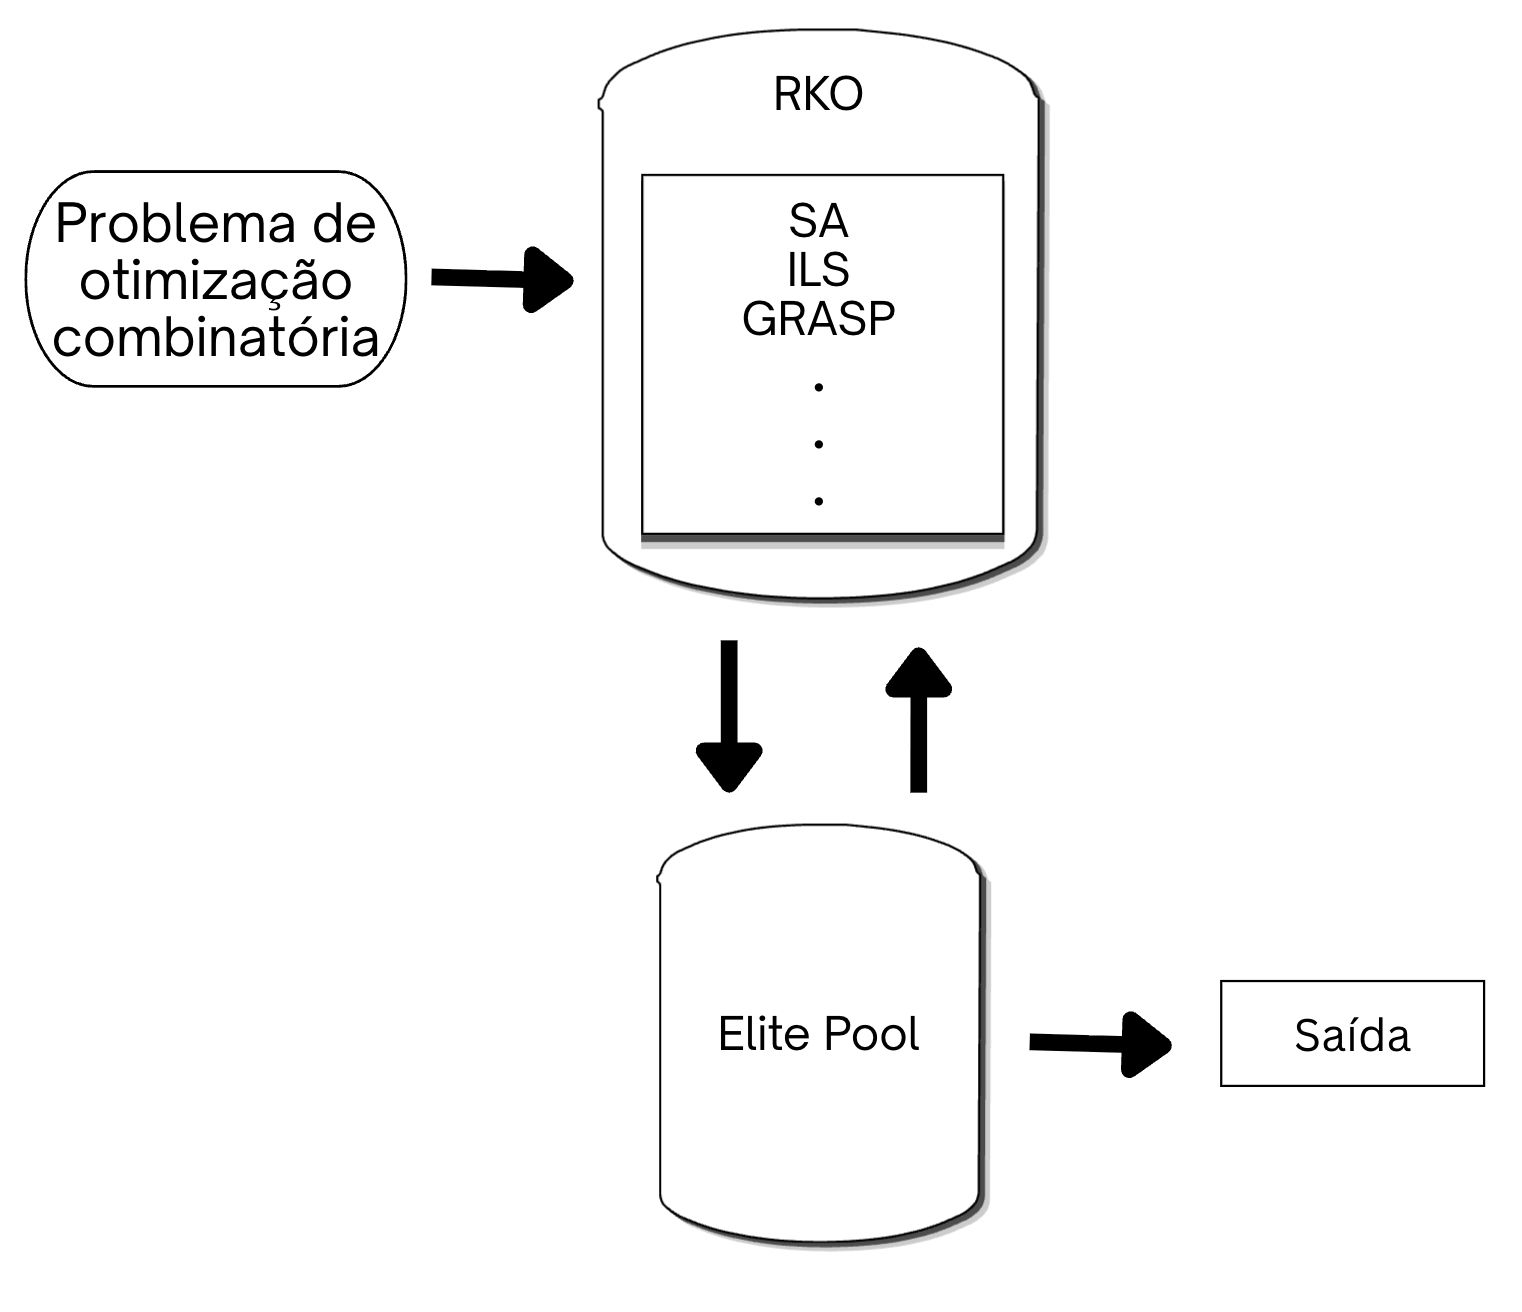
\includegraphics[width=0.6\textwidth]{RKO_Flow.jpeg}
    \caption*{Fonte: autoria própria.}
    \label{fig:RKO_Flow}
\end{figure}

\subsection{Abordagens de otimização da literatura}

Nesta seção, apresentamos as quatro formulações desenvolvidas para o Problema de Compra Mínima (PCmin) proposto por Catabriga~\cite{catabriga2025}. Conforme demonstrado no Teorema 2 do referido trabalho, o espaço de busca dos preços pode ser significativamente reduzido sem perda de otimalidade, restringindo-se ao conjunto de preços candidatos $P_i = \{v_{ib} \mid \forall b \in B\} \setminus \{0\} \cup \{R_i\}$. Tal resultado é fundamental, pois permite limitar o domínio das variáveis de preço a um conjunto finito e relevante, reduzindo o tamanho das formulações e melhorando sua tratabilidade computacional.

\subsubsection{Formulação de Decisão Indireta Binária (DIB)}

Proposta originalmente por Aggarwal et al.~\cite{aggarwal2004} para o problema de maximização (PCmax) e posteriormente adaptada neste trabalho para o contexto do PCmin, a formulação DIB adota uma abordagem de decisão indireta. Nessa modelagem, os preços dos itens são explicitamente representados por variáveis de decisão, enquanto a alocação entre itens e compradores não é modelada de forma direta, sendo inferida a partir das decisões de pagamento.

As variáveis binárias desempenham papel central na formulação. A variável $x_{ip}$ assume valor 1 caso o item $i$ seja precificado com o valor $p$, e 0 caso contrário, representando assim a decisão de atribuição de preços aos itens. Por sua vez, a variável $y_{bp}$ assume valor 1 se o comprador $b$ realiza uma compra pagando o preço $p$, e 0 caso contrário, modelando diretamente o comportamento de pagamento dos compradores.

\begin{align}
\text{maximizar} \quad & \sum_{b \in B} \sum_{p \in P} p \cdot y_{bp} \label{dib_obj} \\
\text{sujeito a} \quad & \sum_{p \in P} x_{ip} \leq 1, & \forall i \in I \label{dib_1} \\
& y_{bp} \leq \sum_{i \in I: v_{ib} \geq p} x_{ip}, & \forall b \in B, \forall p \in P \label{dib_2} \\
& \sum_{p \in P} y_{bp} \leq 1, & \forall b \in B \label{dib_3} \\
& \sum_{p' \in P: p' < p, p' \leq v_{ib}} x_{ip'} \leq 1 - y_{bp}, & \forall b \in B, \forall i \in I, \forall p \in P \label{dib_pcm} \\
& y_{bp}, x_{ip} \in \{0, 1\}, & \forall b \in B, \forall i \in I, \forall p \in P \label{dib_dom}
\end{align}

A função objetivo \eqref{dib_obj} maximiza a receita total obtida a partir dos compradores, somando os valores pagos em cada transação. Como as variáveis $y_{bp}$ indicam diretamente se um comprador realiza um pagamento de valor $p$, a função objetivo captura de forma explícita o total arrecadado.

A restrição \eqref{dib_1} garante que cada item receba no máximo um preço. Embora não se imponha explicitamente que todo item deva ser precificado, a própria estrutura de maximização da receita favorece a atribuição de preços àqueles itens que possam contribuir para a função objetivo.

A restrição \eqref{dib_2} estabelece a ligação entre os preços definidos e os pagamentos realizados. Especificamente, ela assegura que um comprador só pode pagar um determinado preço $p$ se existir ao menos um item precificado com esse valor e cuja valoração para esse comprador seja suficiente para justificar a compra. Dessa forma, embora a alocação não seja explicitamente modelada, essa restrição garante sua consistência implícita.

A restrição \eqref{dib_3} impõe que cada comprador realize no máximo uma compra, refletindo a hipótese de demanda unitária. Isso impede que um mesmo comprador contribua múltiplas vezes para a receita total, mantendo coerência com a estrutura do problema.

A restrição \eqref{dib_pcm} é o principal elemento que adapta a formulação ao contexto do PCmin. Ela garante que, caso um comprador $b$ pague o preço $p$, então não exista qualquer item disponível para esse comprador com preço estritamente menor que $p$. Em outras palavras, essa restrição força que o pagamento realizado corresponda ao menor preço dentre todos os itens que o comprador pode adquirir, modelando diretamente o comportamento racional de escolha do item mais barato.

Por fim, as restrições de domínio \eqref{dib_dom} definem a natureza binária das variáveis de decisão, assegurando que tanto a atribuição de preços quanto as decisões de pagamento sejam modeladas de forma discreta.

Em conjunto, a formulação modela o problema ao integrar decisões de precificação e comportamento dos compradores de maneira consistente: os preços são atribuídos aos itens, os compradores escolhem pagar por no máximo um item compatível com sua valoração, e a estrutura de restrições garante que essa escolha corresponda sempre ao menor preço disponível. Assim, mesmo sem explicitar diretamente a alocação item-comprador, a formulação consegue representar fielmente a dinâmica do problema de compra mínima.

\subsubsection{Formulação de Decisão Direta (DD)}

A formulação DD adota uma abordagem de decisão direta, combinando variáveis binárias de alocação com variáveis contínuas de preço. Diferentemente da formulação indireta, essa modelagem representa explicitamente a relação entre compradores e itens, permitindo capturar de forma mais direta a estrutura do problema. Ao mesmo tempo, a utilização de variáveis contínuas para os preços confere maior flexibilidade à modelagem.

As variáveis de decisão são definidas da seguinte forma: $x_{ib}$ é uma variável binária que indica se o comprador $b$ adquire o item $i$; $\hat{p}_{ib}$ representa o valor efetivamente pago por $b$ ao adquirir $i$; $\pi_i$ corresponde ao preço atribuído ao item $i$; e $y{ib}$ é uma variável binária que indica se o item $i$ é viável para o comprador $b$, isto é, se seu preço é compatível com a valoração $v_{ib}$.

\begin{align}
\text{maximizar} \quad & \sum_{b \in B} \sum_{i \in S_b} \hat{p}_{ib} \label{dd_obj} \\
\text{sujeito a} \quad & \sum_{i \in S_b} x_{ib} \leq 1, & \forall b \in B \label{dd_1} \\
& v_{ib} \cdot x_{ib} - \hat{p}_{ib} \geq 0, & \forall b \in B, \forall i \in S_b \label{dd_2} \\
& \hat{p}_{ib} \leq \pi_i, & \forall b \in B, \forall i \in S_b \label{dd_3} \\
& \hat{p}_{ib} \geq \pi_i - R_i \cdot (1 - x_{ib}), & \forall b \in B, \forall i \in S_b \label{dd_4}  \\
& y_{ib} \geq \frac{v_{ib} - \pi_i + \epsilon}{v_{ib} + \epsilon}, & \forall b \in B, \forall i \in S_b \label{dd_viab}  \\
& \pi_i \geq \sum_{j \in S_b} \hat{p}_{jb} - R_b(1 - y_{ib}), & \forall b \in B, \forall i \in S_b \label{dd_pcm}  \\
& \hat{p}_{ib} \geq 0, & \forall b \in B, \forall i \in S_b \label{dd_5} \\
& \pi_i \geq 0, & \forall i \in I \label{dd_6}  \\
& x_{ib}, y_{ib} \in \{0, 1\}, & \forall b \in B, \forall i \in S_b \label{dd_7} 
\end{align}

A função objetivo \eqref{dd_obj} maximiza a receita total obtida, somando os valores efetivamente pagos pelos compradores. Como $\hat{p}_{ib}$ representa diretamente o pagamento associado à alocação do item $i$ ao comprador $b$, a função objetivo captura explicitamente o valor arrecadado pela solução.

A restrição \eqref{dd_1} garante que cada comprador seja alocado a no máximo um item, refletindo a hipótese de demanda unitária. Assim, evita-se que um mesmo comprador realize múltiplas compras.

A restrição \eqref{dd_2} assegura que o pagamento realizado por um comprador não exceda sua valoração pelo item adquirido. Caso $x_{ib} = 1$, a desigualdade impõe $\hat{p}{ib} \leq v{ib}$; caso contrário, a restrição não impõe limite relevante, sendo posteriormente controlada pelas demais restrições.

As restrições \eqref{dd_3} e \eqref{dd_4} atuam em conjunto para vincular o pagamento ao preço do item. A restrição \eqref{dd_3} garante que o valor pago por um comprador não ultrapasse o preço $\pi_i$ do item. Já a restrição \eqref{dd_4}, por meio de um parâmetro grande $R_i$, força que, sempre que $x_{ib} = 1$, o pagamento $\hat{p}_{ib}$ seja igual ao preço $\pi_i$. Quando $x{ib} = 0$, essa restrição é relaxada, permitindo que $\hat{p}_{ib}$ assuma valor nulo. Dessa forma, essas duas restrições asseguram consistência entre preço e pagamento apenas quando há alocação.

A restrição \eqref{dd_viab} define a variável binária $y_{ib}$ como um indicador de viabilidade. Quando o preço do item $i$ é menor ou igual à valoração $v_{ib}$, o lado direito da desigualdade aproxima-se de 1, forçando $y_{ib} = 1$. Caso contrário, o lado direito torna-se inferior a 1, permitindo que $y_{ib}$ assuma valor 0. Assim, essa restrição identifica corretamente os pares item-comprador para os quais a compra é factível.

A restrição \eqref{dd_pcm} é responsável por modelar a condição de compra mínima. Quando um item $i$ é viável para o comprador $b$ (isto é, $y_{ib} = 1$), a restrição impõe que seu preço $\pi_i$ seja maior ou igual ao valor pago por $b$. Como a função objetivo maximiza esse pagamento, o modelo é induzido a igualar esse valor ao menor preço dentre todos os itens viáveis para o comprador, garantindo o comportamento racional de escolha do item mais barato. Caso o item não seja viável ($y_{ib} = 0$), a restrição é relaxada por meio do termo $R_b(1 - y_{ib})$.

As restrições \eqref{dd_5} e \eqref{dd_6} garantem a não negatividade das variáveis de preço e pagamento, enquanto \eqref{dd_7} define a natureza binária das variáveis de decisão $x_{ib}$ e $y_{ib}$.

Em conjunto, a formulação modela o problema ao integrar explicitamente decisões de alocação, precificação e viabilidade. A presença simultânea dessas componentes permite representar de forma direta o processo de decisão dos compradores, assegurando que cada um selecione, dentre os itens viáveis, aquele de menor preço, ao mesmo tempo em que se maximiza a receita total obtida.

\subsubsection{Formulação de Decisão Indireta por Viabilidade (DIV)}

A formulação DIV simplifica a modelagem ao eliminar variáveis de alocação explícita, concentrando-se exclusivamente na relação entre viabilidade dos itens e o preço efetivamente pago por cada comprador. Diferentemente da formulação DD, não há uma variável que indique diretamente qual item foi escolhido; essa decisão é inferida implicitamente a partir das restrições do modelo.

As variáveis de decisão são definidas como segue: $\pi_i$ representa o preço atribuído ao item $i$; $\hat{p}b$ denota o valor pago pelo comprador $b$; e $y{ib}$ é uma variável binária que indica se o item $i$ é viável para o comprador $b$, ou seja, se o preço do item é compatível com sua valoração $v_{ib}$.

\begin{align}
\text{maximizar} \quad & \sum_{b \in B} \hat{p}_b \label{div_obj} \\
\text{sujeito a} \quad & y_{ib} \geq \frac{v_{ib} - \pi_i + \epsilon}{v_{ib} + \epsilon}, & \forall b \in B, \forall i \in S_b \label{div_viab}\\
& \pi_i - v_{ib} \leq (R_i - v_{ib}) \cdot (1 - y_{ib}), & \forall b \in B, \forall i \in S_b \label{div_1} \\
& \hat{p}_b \leq \pi_i + R_b(1 - y_{ib}), & \forall b \in B, \forall i \in S_b \label{div_pcm} \\
& \hat{p}_b \leq \sum_{i \in S_b} (v_{ib} \cdot y_{ib}), & \forall b \in B \label{div_2} \\
& \pi_i \geq 0, & \forall i \in I  \\
& \hat{p}_b \geq 0, & \forall b \in B  \\
& y_{ib} \in \{0, 1\}, & \forall b \in B, \forall i \in S_b 
\end{align}

A função objetivo \eqref{div_obj} maximiza a receita total obtida, somando os valores pagos por cada comprador. Como $\hat{p}_b$ representa diretamente o pagamento realizado por $b$, a função objetivo captura o valor arrecadado de forma agregada, sem explicitar qual item foi adquirido.

As restrições \eqref{div_viab} e \eqref{div_1} atuam conjuntamente para definir a viabilidade dos itens. A restrição \eqref{div_viab} força a variável $y_{ib}$ a assumir valor 1 quando o preço do item $i$ é menor ou igual à valoração $v_{ib}$, enquanto a restrição \eqref{div_1} garante que, sempre que $y_{ib} = 1$, tem-se $\pi_i \leq v_{ib}$. Dessa forma, essas duas restrições asseguram que $y_{ib}$ identifica corretamente os itens acessíveis a cada comprador.

A restrição \eqref{div_pcm} modela a condição de compra mínima. Para cada item viável ($y_{ib} = 1$), essa restrição impõe que o valor pago $\hat{p}_b$ não exceda o preço $\pi_i$. Como isso vale para todos os itens viáveis, $\hat{p}_b$ é limitado superiormente pelo menor preço dentre eles.

A restrição \eqref{div_2} reforça a consistência econômica do modelo ao garantir que o valor pago por um comprador não exceda sua valoração pelos itens viáveis. Assim, evita-se que o modelo produza soluções em que um comprador pague mais do que estaria disposto a pagar.

As restrições restantes asseguram a não negatividade das variáveis contínuas e a natureza binária das variáveis $y_{ib}$.

Em conjunto, a formulação modela o problema de forma implícita: embora não haja uma variável que identifique diretamente o item escolhido, as restrições impõem que o valor $\hat{p}_b$ corresponda ao menor preço dentre os itens viáveis para cada comprador. Como a função objetivo busca maximizar esse valor, o modelo reproduz corretamente o comportamento racional dos compradores no problema de compra mínima, ao mesmo tempo em que reduz o número de variáveis e simplifica a estrutura da formulação.

\subsubsection{Formulação de Decisão Direta e por Inveja (DDI)}

A formulação DDI baseia-se no conceito de \textit{envy-free pricing}, explorando relações entre compradores para impor limites consistentes sobre os preços pagos. Diferentemente das formulações anteriores, essa abordagem não modela explicitamente preços por item, mas sim utiliza comparações entre valorações de diferentes compradores para garantir coerência econômica na solução.

As variáveis de decisão são definidas da seguinte forma: $x_{ib}$ é uma variável binária que indica se o comprador $b$ é alocado ao item $i$, enquanto $\hat{p}_b$ representa o valor pago pelo comprador $b$. Assim como em outras formulações, assume-se que cada comprador pode adquirir no máximo um item.

\begin{align}
\text{maximizar} \quad & \sum_{b \in B} \hat{p}_b \label{ddi_obj} \\
\text{sujeito a} \quad & \sum_{i \in S_b} x_{ib} \leq 1, & \forall b \in B \label{ddi_1} \\
& \hat{p}_b \leq v_{ib'} + R_b \cdot (1 - x_{ib'}), & \forall b \in B, \forall i \in S_b, \forall b' \in S_i \wedge v_{ib'} \leq v_{ib} \label{ddi_pcm} \\
& \hat{p}_b \leq \sum_{i \in S_b} (v_{ib} \cdot x_{ib}), & \forall b \in B \label{ddi_2} \\
& \hat{p}_b \geq 0, & \forall b \in B  \\
& x_{ib} \in \{0, 1\}, & \forall b \in B, \forall i \in S_b
\end{align}

A função objetivo \eqref{ddi_obj} maximiza a receita total obtida, somando os valores pagos por cada comprador. Como $\hat{p}_b$ representa diretamente o pagamento realizado, a função objetivo agrega a contribuição individual de cada comprador para o valor total arrecadado.

A restrição \eqref{ddi_1} impõe que cada comprador seja alocado a no máximo um item, preservando a hipótese de demanda unitária e evitando múltiplas aquisições por um mesmo comprador.

A restrição \eqref{ddi_pcm} é o elemento central da formulação e incorpora o conceito de \textit{envy-free pricing}. Ela estabelece que o valor pago por um comprador $b$ não pode exceder a valoração de outro comprador $b'$ para um mesmo item $i$, sempre que essa valoração for menor ou igual à de $b$. Intuitivamente, isso impede que um comprador pague mais por um item enquanto outro comprador estaria disposto a adquiri-lo por um valor inferior, evitando situações de “inveja”. O termo com constante grande $R_b$ garante que essa restrição seja ativada apenas quando o item $i$ está efetivamente associado ao comprador considerado.

A restrição \eqref{ddi_2} assegura a consistência entre o pagamento realizado e a valoração do item efetivamente escolhido. Como $x_{ib}$ indica a alocação, essa restrição garante que o valor pago por $b$ não ultrapasse sua valoração pelo item adquirido.

As demais restrições definem a não negatividade das variáveis de pagamento e a natureza binária das decisões de alocação.

Em conjunto, a formulação modela o problema ao explorar relações globais entre compradores, ao invés de depender exclusivamente de decisões locais de preço ou viabilidade. As restrições de \textit{envy-free pricing} garantem que os pagamentos sejam consistentes com a estrutura de preferências dos compradores, evitando soluções em que algum agente teria incentivo a escolher uma alternativa mais barata. Dessa forma, mesmo sem explicitar diretamente os preços dos itens, a formulação assegura que cada comprador paga um valor compatível com o menor preço possível dentre as opções disponíveis, caracterizando adequadamente o problema de compra mínima.

As quatro formulações apresentadas diferem principalmente na forma como modelam as decisões de preço, alocação e viabilidade, o que impacta diretamente tanto o tamanho quanto a força de suas relaxações lineares. A formulação DIB, por adotar uma abordagem indireta com variáveis binárias para preços e pagamentos, tende a produzir modelos mais compactos em termos de alocação explícita, porém com um número potencialmente elevado de variáveis associadas ao conjunto de preços candidatos. Por outro lado, a formulação DD modela explicitamente a alocação entre compradores e itens, o que a torna mais intuitiva e estruturalmente fiel ao problema, mas ao custo de um maior número de variáveis e restrições.

A formulação DIV surge como uma simplificação da DD, eliminando variáveis de alocação e concentrando-se na modelagem da viabilidade e do preço mínimo pago. Essa redução resulta em modelos mais enxutos, embora dependa fortemente da função objetivo para induzir corretamente o comportamento de escolha do menor preço. Já a formulação DDI explora relações entre compradores por meio do conceito de \textit{envy-free pricing}, introduzindo restrições globais que capturam comparações entre diferentes agentes, o que pode fortalecer a formulação ao restringir soluções inconsistentes.

De maneira geral, formulações com decisão direta tendem a oferecer maior controle estrutural sobre a solução, enquanto formulações indiretas frequentemente resultam em modelos menores e potencialmente mais eficientes computacionalmente. A escolha da formulação mais adequada depende, portanto, de um equilíbrio entre tamanho do modelo, força da relaxação linear e desempenho prático observado na resolução das instâncias.

\section{Objetivos}

O presente trabalho tem como objetivo principal investigar e propor melhorias nas formulações matemáticas existentes para o problema de compra mínima, com foco no aprimoramento de sua consistência estrutural e eficiência computacional. Em particular, busca-se desenvolver variações das formulações apresentadas que resultem em modelos mais fortes do ponto de vista de relaxação linear e, consequentemente, mais eficientes quando resolvidos por solvers de otimização modernos.

Nesse contexto, pretende-se analisar criticamente as formulações DIB, DD, DIV e DDI, identificando possíveis fragilidades, redundâncias ou oportunidades de fortalecimento por meio da introdução de novas restrições, reformulações ou técnicas de linearização. O objetivo é obter modelos que apresentem melhor desempenho prático, reduzindo o tempo de resolução e melhorando a qualidade dos limites obtidos por métodos exatos, especialmente quando utilizados em ferramentas como o solver Gurobi~\cite{gurobi}.

Adicionalmente, este trabalho visa abordar o desafio da escalabilidade, propondo abordagens heurísticas capazes de lidar com instâncias de grande porte, envolvendo mais de mil itens ou compradores. Para isso, serão desenvolvidas e avaliadas heurísticas baseadas no Algoritmo Genético de Chaves Aleatórias Enviésadas e na abordagem Otimizador de Chaves Aleatórias, explorando sua capacidade de produzir soluções de boa qualidade em tempos computacionais reduzidos.

Por fim, espera-se que a combinação entre melhorias nas formulações exatas e o desenvolvimento de métodos heurísticos contribua para ampliar a aplicabilidade prática do problema estudado, permitindo a resolução eficiente de instâncias que são desafiadoras para abordagens puramente exatas.
\section{Plano de Trabalho e Cronograma de atividades}

O plano de trabalho deste projeto contempla a realização de disciplinas obrigatórias exigidas pelo programa de pós-graduação, bem como o desenvolvimento das etapas de pesquisa ao longo dos anos de 2026 e 2027. No primeiro ano, estão previstas atividades acadêmicas relacionadas ao cumprimento de créditos, distribuídas ao longo de todos os trimestres de 2026.

Paralelamente, será conduzida uma revisão bibliográfica inicial nos dois primeiros trimestres de 2026, com o objetivo de fundamentar teoricamente o problema abordado. Essa revisão será continuamente atualizada ao longo do desenvolvimento do projeto, conforme novos avanços relevantes na literatura.

Ainda no primeiro ano, está prevista a realização do Exame de Qualificação de Mestrado (EQM) no terceiro trimestre de 2026, momento no qual serão apresentadas as definições formais do problema, a modelagem proposta e possíveis resultados preliminares.

Adicionalmente, o candidato participará do Programa de Estágio Docente (PED) entre o terceiro e o quarto trimestres de 2026, visando à aquisição de experiência em atividades de ensino e apoio acadêmico.

No que diz respeito ao desenvolvimento científico do projeto, as melhorias nas formulações matemáticas serão realizadas entre o terceiro e o quarto trimestres de 2026, período em que também ocorrerá a consolidação dos modelos propostos.

No segundo ano, está prevista a realização de um estágio de pesquisa no exterior por meio do programa de Bolsa
Estágio de Pesquisa no Exterior (BEPE), a ser desenvolvido ao longo dos dois primeiros trimestres de 2027. Esse estágio tem como objetivo fortalecer a colaboração internacional e aprofundar aspectos teóricos e computacionais do trabalho.

Ainda em 2027, serão desenvolvidas heurísticas baseadas em BRKGA e RKO durante o primeiro semestre, com foco na resolução de instâncias de grande porte. Na sequência, a etapa de experimentação computacional será conduzida no terceiro trimestre, permitindo a avaliação de desempenho dos modelos e métodos propostos.

A análise dos resultados obtidos dará suporte à escrita e submissão de artigos científicos, previstas para o terceiro trimestres de 2027. Por fim, a redação da dissertação será realizada entre o terceiro e o quarto trimestres, culminando na entrega e defesa do trabalho ao final de 2027. A Tabela~\ref{cronograma} demonstra como estas etapas estão distribuídas ao longo do período de desenvolvimento do projeto.

\begin{table}[H]
\caption{Cronograma trimestral do projeto de Mestrado}
\label{cronograma}
\centering
\begin{adjustbox}{width=\textwidth}
\begin{tabular}{|l|cllcllcllcll|cllcllcllcll|}
\hline
                                                   & \multicolumn{12}{c|}{\textbf{2026}}                                                                                                                           & \multicolumn{12}{c|}{\textbf{2027}}                                                                                                                           \\ \hline
                                                   & \multicolumn{3}{c|}{\textbf{Jan-Mar}} & \multicolumn{3}{c|}{\textbf{Abr-Jun}} & \multicolumn{3}{c|}{\textbf{Jul-Set}} & \multicolumn{3}{c|}{\textbf{Out-Dez}} & \multicolumn{3}{c|}{\textbf{Jan-Mar}} & \multicolumn{3}{c|}{\textbf{Abr-Jun}} & \multicolumn{3}{c|}{\textbf{Jul-Set}} & \multicolumn{3}{c|}{\textbf{Out-Dez}} \\ \hline
Disciplinas                                        & \multicolumn{3}{c|}{•}                & \multicolumn{3}{c|}{•}                & \multicolumn{3}{c|}{•}                & \multicolumn{3}{c|}{•}                & \multicolumn{3}{c|}{}                 & \multicolumn{3}{c|}{}                 & \multicolumn{3}{c|}{}                 & \multicolumn{3}{c|}{}                 \\ \hline
EQM                                                & \multicolumn{3}{c|}{}                 & \multicolumn{3}{c|}{}                 & \multicolumn{3}{c|}{•}                & \multicolumn{3}{c|}{}                 & \multicolumn{3}{c|}{}                 & \multicolumn{3}{c|}{}                 & \multicolumn{3}{c|}{}                 & \multicolumn{3}{c|}{}                 \\ \hline
Revisão bibliográfica                              & \multicolumn{3}{c|}{•}                & \multicolumn{3}{c|}{•}                & \multicolumn{3}{c|}{•}                 & \multicolumn{3}{c|}{•}                 & \multicolumn{3}{c|}{•}                 & \multicolumn{3}{c|}{•}                 & \multicolumn{3}{c|}{•}                 & \multicolumn{3}{c|}{•}                 \\ \hline
BEPE                                               & \multicolumn{3}{c|}{}                 & \multicolumn{3}{c|}{}                 & \multicolumn{3}{c|}{}                 & \multicolumn{3}{c|}{}                 & \multicolumn{3}{c|}{•}                & \multicolumn{3}{c|}{•}                & \multicolumn{3}{c|}{}                 & \multicolumn{3}{c|}{}                 \\ \hline
PED                                                & \multicolumn{3}{c|}{}                 & \multicolumn{3}{c|}{}                 & \multicolumn{3}{c|}{•}                & \multicolumn{3}{c|}{•}                & \multicolumn{3}{c|}{}                 & \multicolumn{3}{c|}{}                 & \multicolumn{3}{c|}{}                 & \multicolumn{3}{c|}{}                 \\ \hline
Melhorias nas formulações                          & \multicolumn{3}{c|}{}                 & \multicolumn{3}{c|}{}                 & \multicolumn{3}{c|}{•}                & \multicolumn{3}{c|}{•}                & \multicolumn{3}{c|}{}                 & \multicolumn{3}{c|}{}                 & \multicolumn{3}{c|}{}                 & \multicolumn{3}{c|}{}                 \\ \hline
Desenvolvimento de heurísticas                     & \multicolumn{3}{c|}{}                 & \multicolumn{3}{c|}{}                 & \multicolumn{3}{c|}{}                 & \multicolumn{3}{c|}{}                 & \multicolumn{3}{c|}{•}                & \multicolumn{3}{c|}{•}                & \multicolumn{3}{c|}{}                 & \multicolumn{3}{c|}{}                 \\ \hline
Experimentação computacional & \multicolumn{3}{c|}{}                 & \multicolumn{3}{c|}{}                 & \multicolumn{3}{c|}{}                 & \multicolumn{3}{c|}{}                 & \multicolumn{3}{c|}{}                 & \multicolumn{3}{c|}{}                 & \multicolumn{3}{c|}{•}                & \multicolumn{3}{c|}{}                 \\ \hline
Escrita de artigos cientifícos                     & \multicolumn{3}{c|}{}                 & \multicolumn{3}{c|}{}                 & \multicolumn{3}{c|}{}                 & \multicolumn{3}{c|}{}                 & \multicolumn{3}{c|}{}                 & \multicolumn{3}{c|}{}                & \multicolumn{3}{c|}{•}                & \multicolumn{3}{c|}{}                 \\ \hline
Escrita da dissertação                             & \multicolumn{3}{c|}{}                 & \multicolumn{3}{c|}{}                 & \multicolumn{3}{c|}{}                 & \multicolumn{3}{c|}{}                 & \multicolumn{3}{c|}{}                 & \multicolumn{3}{c|}{}                 & \multicolumn{3}{c|}{•}                & \multicolumn{3}{c|}{•}                \\ \hline
Entrega da dissertação e defesa                    & \multicolumn{3}{c|}{}                 & \multicolumn{3}{c|}{}                 & \multicolumn{3}{c|}{}                 & \multicolumn{3}{c|}{}                 & \multicolumn{3}{c|}{}                 & \multicolumn{3}{c|}{}                 & \multicolumn{3}{c|}{}                 & \multicolumn{3}{c|}{•}                \\ \hline
\end{tabular}
\end{adjustbox}
\end{table}
\section{Materiais e Métodos}

O presente projeto será desenvolvido nas dependências do Laboratório de Otimização e Combinatória (LOCo) do Instituto de Computação, um ambiente compartilhado com outros estudantes de mestrado e doutorado que propicia a troca de ideias e a colaboração científica. Os algoritmos propostos serão testados empiricamente. Devido ao grande volume de instâncias disponíveis na literatura e aos elevados limites de tempo comumente adotados em trabalhos anteriores (frequentemente estabelecidos em uma hora por execução), as baterias de testes podem demandar dias para serem concluídas. Por essa razão, os experimentos computacionais serão executados nos servidores de alto desempenho disponibilizados pelo LOCo.

Para o suporte teórico e o levantamento do estado da arte, o candidato utilizará o acervo bibliográfico físico da biblioteca do Instituto de Matemática, Estatística e Computação Científica, além do Portal de Periódicos da CAPES, que assegura acesso institucional e gratuito às principais revistas científicas da área para os estudantes da Unicamp.

A metodologia de acompanhamento incluirá reuniões entre o candidato e o orientador para debater o andamento da pesquisa, superar desafios metodológicos e alinhar novas estratégias de resolução. Adicionalmente, encontros com os demais membros do grupo de pesquisa do orientador ocorrerão de forma periódica ou sob demanda, promovendo a integração e a discussão coletiva dos resultados alcançados.
\section{Forma de Análise dos Resultados}

A análise dos resultados deste trabalho será conduzida com o objetivo de avaliar, de forma sistemática, a qualidade e a eficiência das formulações propostas, bem como dos métodos de solução desenvolvidos. Para isso, serão considerados tanto aspectos relacionados à qualidade das soluções obtidas quanto ao desempenho computacional dos algoritmos.

Inicialmente, as formulações matemáticas propostas serão avaliadas por meio de sua capacidade de produzir soluções ótimas ou de alta qualidade dentro de limites de tempo computacional preestabelecidos. Serão analisadas métricas como valor da função objetivo, tempo de processamento e número de nós explorados pelos algoritmos de \emph{branch-and-bound}, quando aplicável. Além disso, será verificada a robustez das formulações em instâncias de diferentes tamanhos, com ênfase especial em problemas de grande porte.

Para a comparação entre os diferentes modelos e abordagens, será utilizada a metodologia de \emph{performance profiles}, conforme proposto por Dolan e Moré~\cite{Dolan2002}. Essa técnica permite avaliar o desempenho relativo dos algoritmos em um conjunto de instâncias, considerando simultaneamente eficiência e robustez. A partir dessa análise, será possível identificar quais formulações e métodos apresentam melhor comportamento geral, bem como aqueles mais adequados para diferentes cenários de aplicação.

No que se refere às heurísticas, serão desenvolvidos e avaliados métodos baseados em BRKGA e RKO, com foco na resolução eficiente de instâncias de grande escala. A qualidade das soluções obtidas por essas heurísticas será comparada com os resultados provenientes dos métodos exatos, considerando tanto o valor da função objetivo quanto o tempo de execução. Sempre que possível, serão utilizados limites inferiores fornecidos pelos modelos exatos para mensurar o \emph{gap} de otimalidade das soluções heurísticas.

Adicionalmente, será investigada a possibilidade de desenvolvimento de heurísticas baseadas nos próprios métodos exatos. Em particular, serão exploradas estratégias que utilizem informações provenientes da relaxação linear, soluções parciais e estruturas identificadas durante o processo de otimização para guiar a construção de soluções factíveis de alta qualidade. Essa abordagem visa combinar a precisão dos métodos exatos com a eficiência das heurísticas, resultando em algoritmos híbridos mais robustos e escaláveis.

Por fim, os resultados obtidos serão analisados de forma comparativa e crítica em artigos cientifícos e na dissertação de mestrado, buscando identificar padrões de desempenho, limitações das abordagens propostas e possíveis direções para trabalhos futuros.

\newpage
\bibliographystyle{plain}
\bibliography{Secoes/Referencias/referencias}
\end{document}